% This is "sig-alternate.tex" V2.0 May 2012
% This file should be compiled with V2.5 of "sig-alternate.cls" May 2012
%
% This example file demonstrates the use of the 'sig-alternate.cls'
% V2.5 LaTeX2e document class file. It is for those submitting
% articles to ACM Conference Proceedings WHO DO NOT WISH TO
% STRICTLY ADHERE TO THE SIGS (PUBS-BOARD-ENDORSED) STYLE.
% The 'sig-alternate.cls' file will produce a similar-looking,
% albeit, 'tighter' paper resulting in, invariably, fewer pages.
%
% ----------------------------------------------------------------------------------------------------------------
% This .tex file (and associated .cls V2.5) produces:
%       1) The Permission Statement
%       2) The Conference (location) Info information
%       3) The Copyright Line with ACM data
%       4) NO page numbers
%
% as against the acm_proc_article-sp.cls file which
% DOES NOT produce 1) thru' 3) above.
%
% Using 'sig-alternate.cls' you have control, however, from within
% the source .tex file, over both the CopyrightYear
% (defaulted to 200X) and the ACM Copyright Data
% (defaulted to X-XXXXX-XX-X/XX/XX).
% e.g.
% \CopyrightYear{2007} will cause 2007 to appear in the copyright line.
% \crdata{0-12345-67-8/90/12} will cause 0-12345-67-8/90/12 to appear in the copyright line.
%
% ---------------------------------------------------------------------------------------------------------------
% This .tex source is an example which *does* use
% the .bib file (from which the .bbl file % is produced).
% REMEMBER HOWEVER: After having produced the .bbl file,
% and prior to final submission, you *NEED* to 'insert'
% your .bbl file into your source .tex file so as to provide
% ONE 'self-contained' source file.
%
% ================= IF YOU HAVE QUESTIONS =======================
% Questions regarding the SIGS styles, SIGS policies and
% procedures, Conferences etc. should be sent to
% Adrienne Griscti (griscti@acm.org)
%
% Technical questions _only_ to
% Gerald Murray (murray@hq.acm.org)
% ===============================================================
%
% For tracking purposes - this is V2.0 - May 2012

\documentclass{sig-alternate}
\usepackage{color}
\usepackage[usenames,dvipsnames]{xcolor}
\usepackage{url}

\newcommand{\TODO}[1]{{\color{red} TODO: #1}}
\newcommand{\gametitle}{{\color{RoyalPurple} Dragon Architect Academy}}

\toappear{Submitted for review.}

\begin{document}
%
% --- Author Metadata here ---
%\conferenceinfo{Foundations of Digital Games (FDG)}{2015}
% \pdfinfo{
% /Title ()
% /Author (Aaron Bauer, Eric Butler, Zoran Popovic) 
% /Subject ()
% /Keywords ()
% }
%\CopyrightYear{2007} % Allows default copyright year (20XX) to be over-ridden - IF NEED BE.
%\crdata{0-12345-67-8/90/01}  % Allows default copyright data (0-89791-88-6/97/05) to be over-ridden - IF NEED BE.
% --- End of Author Metadata ---

\title{Visual Programming and Cube-Coding Gooooodtimes}

\numberofauthors{1}
\author{Anonymized}

% \numberofauthors{1} 
% \author{
% \alignauthor
% Aaron Bauer, Eric Butler, Zoran Popovi\'c\\
%        \affaddr{Center for Game Science}\\
%        \affaddr{Computer Science \& Engineering}\\
%        \affaddr{University of Washington}\\
%        \affaddr{Seattle, WA 98195}
%        \email{\{awb, edbutler\}@cs.washington.edu}
% }

\maketitle
\begin{abstract}
\TODO{classy abstract}
\end{abstract}

% A category with the (minimum) three required fields
\category{K.3.2}{Computers and Education}{Computer and Information Science Education -- Computer science education}

\terms{Design, Human Factors}

\keywords{Game-based learning; computational thinking; programming education}

\section{Introduction}
The past few years have seen many efforts to broaden the reach of computer science education and make it available, and appealing, to more students in more places. 
Many of these projects, including some of the most visible such as Scratch and Code.org's Hour of Code~\cite{codedotorg}, are online programming environments that expose users to basic programming concepts. 
Despite the proliferation of these systems, little work has investigated the design of the structure or content of such systems. 
Comparative studies providing evidence for effective ways of presenting these ideas in this context have been largely absent. 

% As one example, we believe the effects of changes in programming language syntax and semantics on novices need more study. 
% One might ask if there are benefits to evolving the available language elements as a novice progresses, and in which order these elements should become available. 
% What combination of language elements affords beginners the most expressiveness without introducing overwhelming complexity? 
% Another set of questions concern the impact of combining puzzles and an open-ended sandbox. 
% Can puzzles provide sufficient structure and guidance to facilitate productive exploration of a game's concepts in an unstructured sandbox? 
% When and how should the player transition between the two? 
% These and many more topics relating to online programming environments deserve further study, particularly in light of their surging popularity \TODO{footnote about \# of Scratch users/Hour of Code participants?}. 
% In this paper, 

In this paper we present \gametitle{}, an educational game designed to be a tool with which to conduct such studies. 
In \gametitle{}, players use a visual, drag-and-drop programming language to control a dragon in a 3D grid world. 
The visual language is a set of \emph{code blocks} that snap together to form programs. 
The player can move the dragon in three dimensions and have the dragon place and remove cubes of various colors. 
In addition to blocks that control the dragon directly, players can also make use of definite loops and procedures (see Figure~\ref{fig:toolbox}).

\begin{figure}[ht]
  \centering
  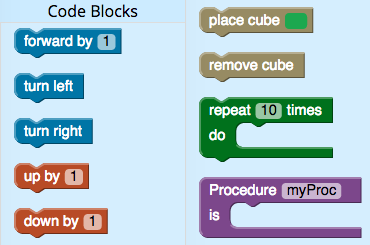
\includegraphics[width=\columnwidth]{images/toolbox_wide}
  \caption{The programming elements currently available in \gametitle{}}
  \label{fig:toolbox}
\end{figure}

Our motivation for developing \gametitle{} is to explore a variety of open questions in both education and games. 
In this paper we review the space of these programming environments and related systems as it currently stands, noting how we differ and how we take inspiration from related work.  
Despite so many existing systems with overlapping educational properties, we developed a new game (as opposed to using existing educational software) in order to design it as a research tool from the ground up.
In Section~\ref{sec:research} we propose four research questions we believe need more study and discuss how these questions have informed the design of our game. 

The remainder of this paper is as follows: after \gametitle{} is described in more detail, it discusses related work and our research goals. 
The paper then highlights several design issues that have arisen during \gametitle{}'s development and presents our observations from students' experiences with the game so far. 
The paper concludes with our thoughts on other interesting questions our game might be used to help answer.

\section{\gametitle{}}
\TODO{Can't use macros in section titles because the formatted gets messed up, replace once we choose a title}
We have been developing \gametitle{} since spring 2014. 
It's played in a web browser, and similar to many other such systems, the page is separated into two parts: an area where the player can assemble their code and a visualization of the environment their code affects (\TODO{figure}). 
The visualization uses the Unity game engine~\TODO{cite} and the drag-and-drop programming UI is provided by the Blockly library~\TODO{cite}.

As they progress through the game, players alternate between short sequences of one to five puzzles with a specific goal and a specific set of available code blocks and an open-ended sandbox. 
The game begins with four puzzles that introduce the idea of assembling and running code, as well as the code blocks for moving the dragon in 2D and putting down cubes.
After that, the player can experiment and build in the sandbox and complete other puzzle sequences to make more code blocks available in the sandbox, switching between sandbox and puzzles at any time. 
Like the first puzzles, each subsequent sequence focuses on a few specific concepts. 
In this way, the language the player uses to write instructions for the dragon gradually expands as the player advances.

\TODO{talk about building on Minecraft's popularity and broad appeal}

% \subsubsection{Language}

% The visual, drag-and-drop language used by the player is a custom, if, in game's development so far, simplistic, language designed specifically for \gametitle{}. We have implemented a textual concrete syntax, and we plan for the game to eventually expose this to the player, allowing them to choose which input method they prefer. This also allows for a direct translation from text to code blocks and vice versa. Some similar projects use a popular industry programming language such as Javascript or Java. We believe implementing our own gives us a valuable flexibility as well as preventing our players from dealing with the idiosyncrasies of any popular language. Having complete control over every part of the language implementation will provide useful in any study of the effects of changes in language features. 

% \subsubsection{Technology}
% \TODO{a few sentences or cut}


\section{Related Work}

\subsection{Learning Theory}
\label{subsec:learning}
Supporters of \emph{constructionism} argue that children can learn through self-directed discovery \TODO{cite} and that this has many advantages over traditional teaching approaches \TODO{cite}.
Others have argued that games are an ideal environment for constructionist teaching \TODO{cite}.
However, evidence suggests that a purely self-directed learning approach is inadquate for effective learning \TODO{cite}.

\subsection{Games and Systems for Computer Science Education}
%The tremendous and recent proliferation, in both quantity and variety, of online programming environments attempting to teach or promote engagement with computer science ideas, especially basic programming concepts, has greatly informed the development of \gametitle{}.
The history of tools designed to teach novices programming dates back to the 1960's, originating with Pappert's LOGO \TODO{cite}.
Kelleher and Pausch review programming environments for novices and describe a taxonomy of these systems~\cite{kelleher2005lowering}.
Within that taxonomy, \gametitle{} fist best as a teaching system that targets \emph{structuring programs} and aims to provide learning support both through \emph{social learning} and \emph{providing a motivating context}.

Lye and Koh recently reviewed studies that investigated teaching computational thinking in K12 classrooms~\cite{lye2014review}.
They found that this area deserves more research.
In particular, the reviewed findings suggest structured, guided discovery is a better approach for learning than pure self-driven discovery.

There a been a recent proliferation of widely available CS education tools on the internet.
In some, like the step-by-step lessons available from Khan Academy~\cite{khanacademy} and Codecademy~\cite{codecademy}, or the game CodeSpells \cite{esper2013codespells}, users program in a popular industry programming language such as Javascript or Java.
Given that syntax can be an obstacle for those new to programming~\cite{stefik2013syntax}, other tools chose to use a visual language as there is evidence those are helpful to novices~\cite{whitley1997visual}.
\TODO{should also mention Programming By Design and related project Bootstrap as curricula-oriented projects}
Examples of such tools include Scratch~\cite{maloney2010scratch}, a visual programming environment focused on empowering its users to create interactive digital media.
Scratch has been successful in building vibrant community around open-ended, creative, social environment (want to borrow ideas of personalization in the future).
Some suggest that the lack of structure may pose a barrier to entry and to learning (quantity and complexity of immediately available features may be intimidating or confusing, discovery-learning-ineffective citation) \TODO{cite};
With \gametitle{}, we want to see if a gradual introduction of features can be easier to get in to while still inspiring the creative experimentation Scratch fostered in its community.

Other recent efforts have, rather than provide an open creative environment, present players with a series of mostly linear challenges.
Many of these examples are games, such as Lighbot \TODO{cite} and \TODO{cite some other example}.
Code.org presents a sequence of explanatory videos and linear puzzles. \TODO{cite}
The project has had extremely wide reach but was limited in scope. \TODO{cite}

Lots of people have tried building upon Minecraft's capacity for broad engagement.
Here's a game from FDG \cite{zorn2013minecraft}.
Here's that project the guy from FDG talked about \TODO{cite}.

\emph{BOTS} is a programming puzzle game. The stated goal of the project is to study how community-athored content is used in educational games~\cite{hickspart14}, and it has also been used to explore hint generation~\TODO{cite}.


\section{Research Questions}
\label{sec:research}
Our primary goal for \gametitle{} is to produce a flexible system that we can use to investigate questions in computer science education and game-based learning. 
Below we present four questions we believe are under-researched and that informed the design of our game. 

\subsection{Scaffolded Sandbox}
Within the context of investigating game-based learning, we believe more research is needed on guided discovery learning to games. 
Some games provide a sandbox where players discover the properties of the environment through largely unguided exploration (e.g. Minecraft, SimCity~\TODO{cite}), and others provide a linear sequence of levels designed to teach the player the relevant information (e.g. Portal~\TODO{cite}). 
In terms of learning theory, the former have a lot in common with pure discovery learning (ignoring potential external sources of information such as wikis or friends), while the latter rely on direct guidance. 

Other games teach players by doing something in between. 
Games in the Zelda series~\TODO{cite} contain a non-linear sequence of puzzles and teach new mechanics by requiring the player demonstrate understanding of a new mechanic before they are allowed to progress. 
Strategy games such as Crusader Kings II~\TODO{cite} offer a set of explicit tutorials the player may choose to go through before beginning more open-ended play.
The variety of approaches games take in teaching players leads to interesting questions about how different methods affect what players do in a game, or, in the case of educational software, how they learn. 
Furthermore, for complex topics such as computer science, the concepts a game needs to teach its players are likely to be more difficult to discover through exploration and require more sophisitcation to explain through direct guidance. Thus, more research is needed to refine and evaluate these techniques. 

Education research indicates that guided discovery learning, the blending of exploration and direct guidance, can benefit learning (see Section~\ref{subsec:learning}). 
In the case of \gametitle{}, we have combined structured puzzle levels and an open, unstructured sandbox. 
The puzzles, by leading the player to demonstrate a particular concept, act as a form of direct guidance. 
A process of discovery can then take place in the sandbox where the player is free to experiment with the ideas introduced in the puzzles. 
As discussed in Section~\ref{sec:action}, our playtesting has shown this approach to be promising for many of the concepts currently in the game. 

\subsection{Compuational Thinking}

Many have studied (e.g. \cite{repenning2010scalable}, \cite{barr2011bringing}) how to increase presence of computational thinking in computer science education (and education in general). \TODO{if you can think of it, you can automate building it = a primary component of Wing's~\cite{wing2008computational} definition of computational thinking --- does this fly in the face of the evidence against discovery learning?}

\TODO{phrase as a question}
It is our goal with \gametitle{} to approach teaching these ideas in a more profound way then simply hoping students absorb this \emph{way of thinking} as a byproduct of working with other computer science concepts (such as basic programming). We propose to go further and teach computational thinking by directly teaching one of its core components: the identification and application of problem-solving strategies (such as divide and conquer). 

A great deal of recent education research suggests that \emph{curricula can model such strategies for students} and that appropriate guidance, which in many cases consists of the capabilities afforded by a suitable computational environment, can \emph{enable students to learn to use these strategies independently}~\cite{report2010computational}. Mayer and Wittrock~\cite{mayer1996handbook} call attention to the substantial evidence in the education literature for teaching what they call \emph{domain-specific thinking skills} and \emph{metacognitive skills}. The former would include the ability to use a strategy like divide and conquer, and the latter would include knowing when and where to employ that strategy. In both cases, studies have shown that teaching these skills directly can improve learning and performance. 

Our goal is to incorporate computational thinking strategies into the content of an educational game. This includes demonstrating these strategies and giving players an opportunity to practice them. We believe a game is particularly well suited to this task. \TODO{expand on this}

\subsection{Language for Novices}
effects of language semantics on novices understudied (other aspects have seen some study --- stefik on syntx, ko on compiler messages)

\subsection{Social Community}
there are examples where social community has been an important part of the success of an online programming environment (e.g. scratch, MOOSE crossing), and research in behavioral and social sciences indicates sharing and collaboration can improve learning~\TODO{cite how people learn book}. Despite this, the specific contributions of social features to an online programming environment remain largely unstudied

\section{Design Issues}

\subsection{Permanence vs. Experimentation}

\subsection{Flexible Puzzles}


\section{\gametitle{} in Action}
\label{sec:action}
\begin{itemize}
\item how we have made our observations
\item what we have observed
\begin{itemize}
\item kids excited by premise
\item some want to do puzzles, some want to play in the sandbox
\item idea generation (i.e. what to do) in the sandbox can be a barrier
\item great interest in personalization
\item often try and accomplish goal bit by bit
\item common confusions: no mental model of code as program, procedure blocks as definition and invocation
\end{itemize}

\item what we have learned from watching \gametitle{} in action
\end{itemize}


\section{Discussion}
\TODO{description of open problems in CS education and game-based learning, exploration of how \gametitle{} might be used to approach them}
\begin{itemize}
\item visual debugging
\item parallel/distributed programming
\item transition to textual representation
\end{itemize}

% Comment out in submission version
%\section{Acknowledgments}
%\TODO{copy from CHI papers?}

\bibliographystyle{abbrv}
\bibliography{ruthefjord-fdg-2015} 
\end{document}
